%\textbf{@Marcello,Francesco: we should also probably elaborate on the kind of verification technique we are using and how that can help in evaluating the topology.. remember here we do not have the DICE restriction so we can mention any kind of analysis that it would be possible to run, also analyses that are currently in the hands of other DICE partners!!}

%\begin{itemize}
%\item we can use the ATC case study as much as we want - that yields already three topologies that we can infer
%\item ATC has agreed that we can mention their role in this exercise, I also showed them the topology that we elicited basically with OSTIA and they already made considerations on how to improve it
%\item in the evaluation we should also comment on how OSTIA can help you in visualizing the application topology that you may be considering to use by reusing a big-data application for something else... visualising the application topology and analysing it may allow you to improve it while you are using it as a starting point for your application
%\item another application that we can use is the one that NETF is considering for their own scenario, KILLRWEATHER - \url{https://github.com/killrweather/killrweather}
%\item any additional case that we can run?
%\item what do the results show? do we have a way to quickly quantify the time that is saved by using this approach? e.g., the time that is saved in setting up and running the infrastructure and how much would that time saved have costed these could be valuable evaluation insights
%\end{itemize}
We evaluated OSTIA through qualitative evaluation and case-study research featuring an open-/closed-source industrial case study (see Section \ref{cs}) and two open-source case studies (see Section \ref{os}) on which we also applied complex formal verification (see Section \ref{ver}).

\subsection{Industrial Case-Study}\label{cs}

%As previously introduced in Section \ref{ra}, 
OSTIA was evaluated using several topologies part of the SocialSensor App. Our industrial partner is having
performance and availability outages connected to currently unknown
circumstances. Therefore, the objective of our evaluation for OSTIA was twofold:
(a) allow our industrial partner to enact continuous architecting of their
application with the goal of discovering any patterns or hotspots that may be
requiring further architectural reasoning; (b) understand whether OSTIA provided
valuable feedback to endure the continuous architecting exercise.

OSTIA standard output\footnote{Output of OSTIA analyses is not evidenced for the
sake of space.} for the smallest of the three SocialSensor topologies, namely
the ``focused-crawler" topology, is outlined in Fig. \ref{topo1}.

\begin{figure*}
\begin{center}
		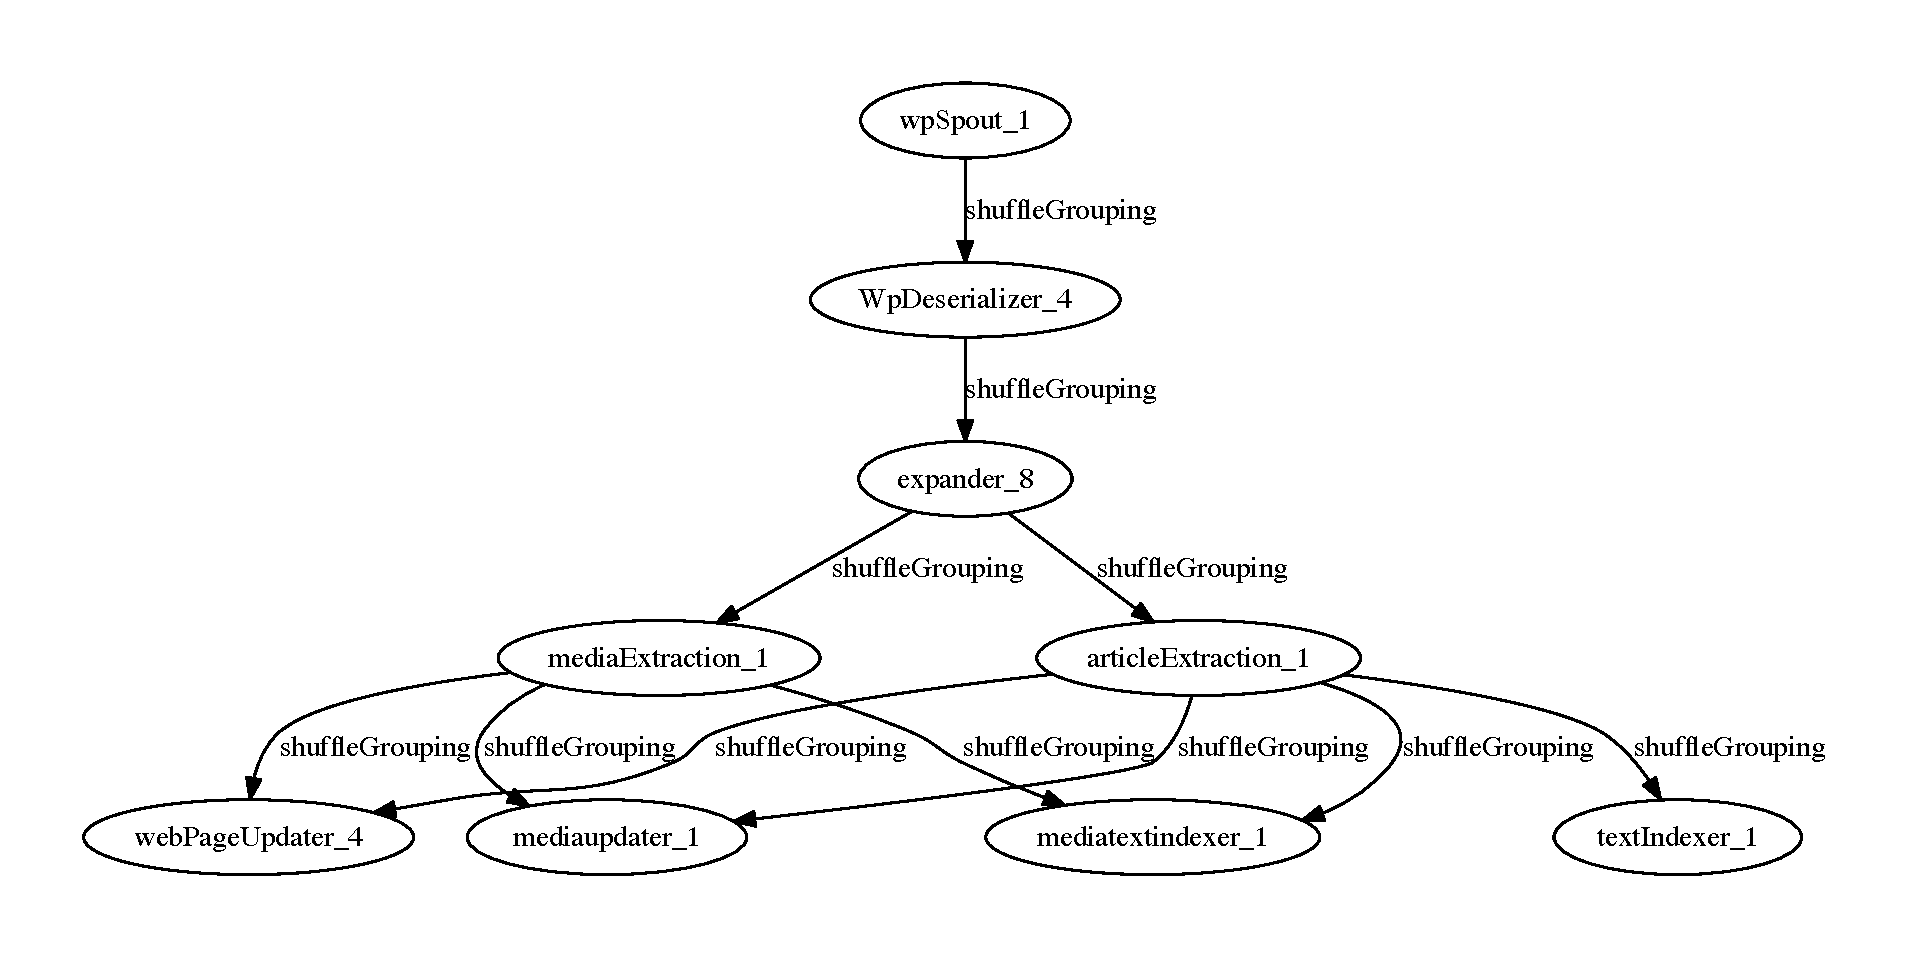
\includegraphics[width=11cm]{images/output/focused_crawler}
		\caption{SocialSensor App, OSTIA sample output.}
		\label{topo1}
		\end{center}
\end{figure*}

OSTIA has been proved particularly helpful in visualising the complex topology
together with the parallelism level of each components. Combining this
information with runtime data, such as latency, our industrial partner observed
that the ``expander" bolt needed additional architectural reasoning. \comment{for example? elaborate more on this. the reviewers will likely say its vague...}
Also, the
partner welcomed the idea of using OSTIA as a mechanism to enact continuous
architecting of the topology in question as part of the needed architectural
reasoning.

Besides this pattern-based evaluation and assessment, OSTIA algorithmic analyses
assisted our client in understanding that the topological structure of the
SocialSensor app would be better fit for batch processing rather than streaming,
since the partner observed autonomously that too many database-output spouts and
bolts were used in their versions of the SocialSensor topologies. In so doing,
the partner is now using OSTIA to drive the refactoring exercise towards a
Hadoop Map Reduce~\cite{hadoop}
%\footnote{\url{http://hadoop.apache.org/}} 
framework for batch processing.

\comment{this section is not good enough, we require to add more information, for example what would be the target architecture after refactoring looks like? we said some patters were idenfitified but we didnt say details of continuous rearchitecting...and also formal verification process for this}

\subsection{Evaluation on Open-Source Software}\label{os}

To confirm the usefulness and capacity of OSTIA to enact a continuous
architecting cycle, we applied it in understanding (first) and attempting
improvements of two open-source applications, namely, the previously introduced
DigitalPebble~\cite{digitalpebble} and 
%\footnote{\url{https://github.com/DigitalPebble}} and
StormCV~\cite{stormCV}
%\footnote{\url{https://github.com/sensorstorm/StormCV}}
applications. Figures \ref{dp} and \ref{scv} outline standard OSTIA output for the two applications. Note that we did not have any prior knowledge concerning the two applications in question and we merely run OSTIA on the applications' codebase dump in our own experimental machine. OSTIA output takes mere seconds for small to medium-sized topologies (e.g., around 25 nodes). 
%
\begin{figure}
\begin{center}
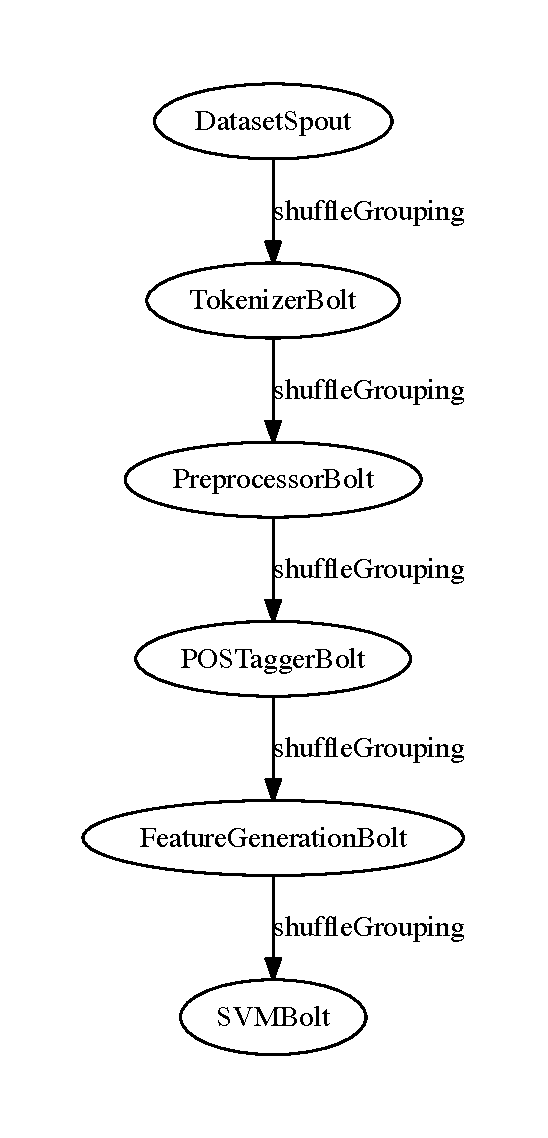
\includegraphics[width=4cm]{images/output/senti_storm}
		\caption{StormCV topology.}
		\label{scv}
		\end{center}
\end{figure}
%%%%
%%%%\begin{figure}
%%%%\label{fig:oscasestudy}
%%%%\centering 
%%%%\subfigure[{\footnotesize DigitalPebble topology.}]{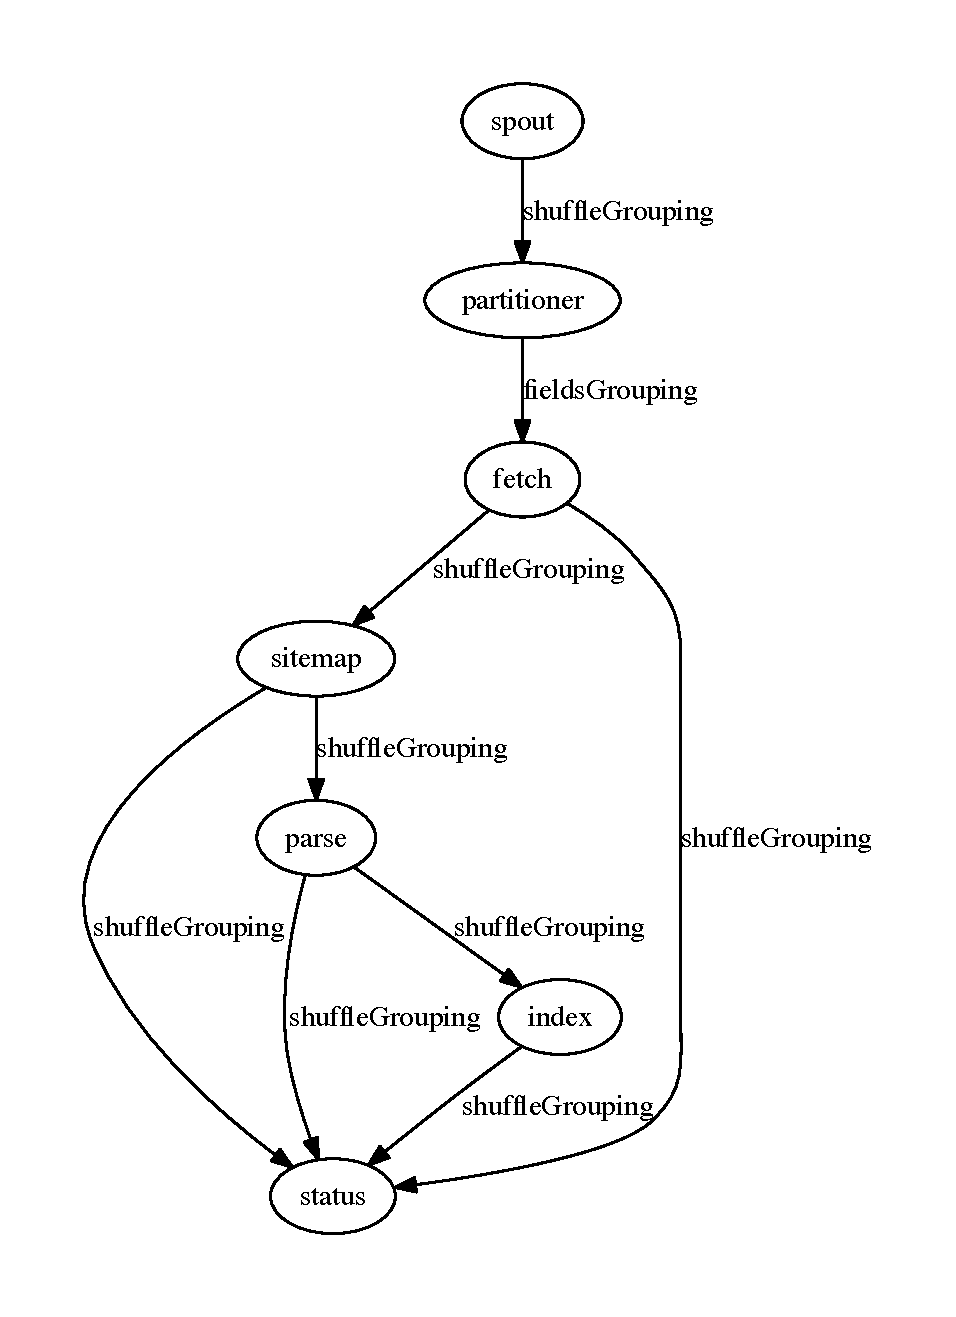
\includegraphics[width=4.5cm]{images/output/crawl}}\label{dp}
%%%%\hspace{0.5cm}
%%%%\subfigure[{\footnotesize StormCV topology.}]{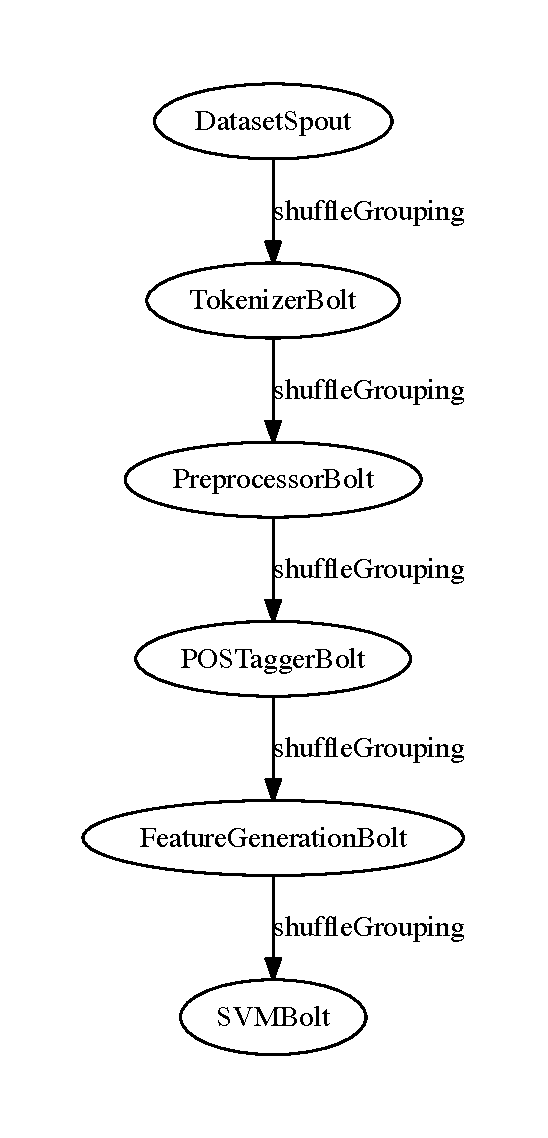
\includegraphics[width=3cm]{images/output/senti_storm}}\label{scv}
%%%%\end{figure}

The OSTIA output aided as follows: (a) the output summarised in Fig. \ref{dp}
allowed us to immediately grasp the functional behavior of the DigitalPebble and
StormCV topologies allowing us to interpret correctly their operations before
reading long documentation or inspecting the code; (b) OSTIA aided us in visually interpreting the complexity of the applications at hand; (c) OSTIA allowed us to spot several anti-patterns in the DigitalPebble Storm application around the ``sitemap" and ``parse" bolts, namely, a multiple cascading instance of the multi-anchoring pattern and a persistent-data pattern. Finally, OSTIA aided in the identification of the computational funnel anti-pattern around the "status" bolt closing the DigitalPebble topology. With this evaluation at hand, developers in the respective communities of DigitalPebble and StormCV could refactor their topologies, e.g., aided by OSTIA-based formal verification that proves the negative effects of said anti-patterns.

\comment{this section needs further elaboration. we need to elaborate our discussion to visually locate these anti patterns.}
% \comment{you said first, where is the second? this is incomplete}
%
%\begin{figure}
%\begin{center}
%		\includegraphics[width=2.7cm]{}
%		\caption{}
%		\label{scv}
%\end{center}
%\end{figure}

\subsection{Continuous Architecting by Means of Formal Verification: An Industrial Case-Study}

In this section we outline the results from OSTIA-based formal verification applied on (one of) the topologies used by our industrial partner in practice. Results provide valuable insights for (re-)architecting and improving these topologies in a continuous manner.

\begin{figure}
\begin{center}
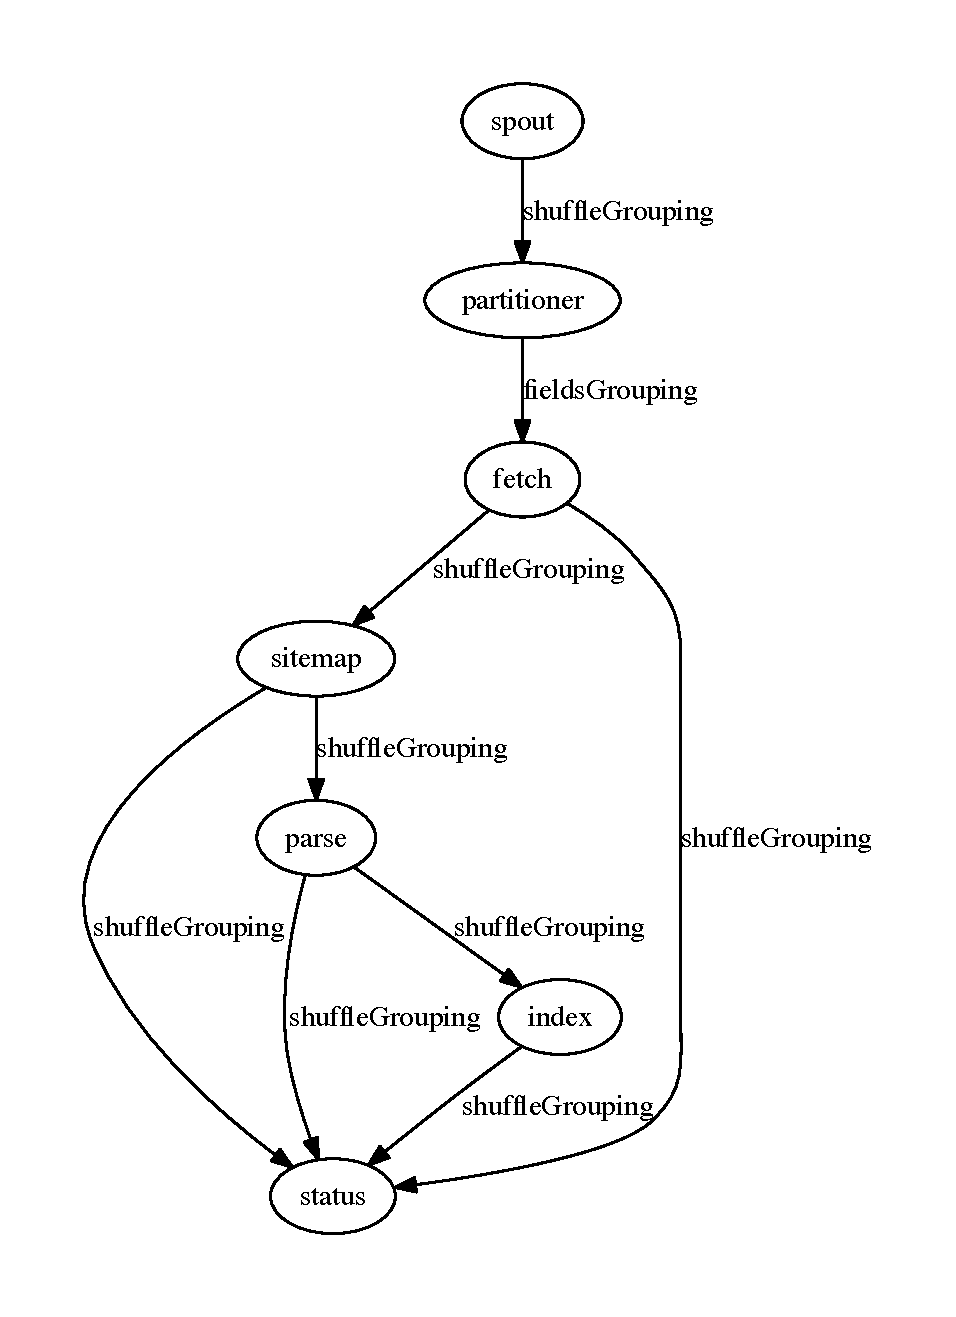
\includegraphics[width=6cm]{images/output/crawl}
		\caption{DigitalPebble topology.}
		\label{dp}
		\end{center}
\end{figure}
The formal analysis of the ``focused-crawler'' topology confirmed the critical role of the ``expander'' bolt, previously noticed with the aim of OSTIA visual output. It emerged from the output traces that there exists an execution of the system, even without failures, where the queue occupation level is unbounded. Figure~\ref{verif-trace} shows how the tool constructed a periodic model in which a suffix (highlighted in red) of a finite sequence of events is repeated infinitely many times after a prefix (in white). After ensuring that the trace is not a spurious model, we concluded that the expander queue, having an increasing trend in the suffix, is unbounded.

\comment{discuss thge benefit of this, was it possible without formal verification?  elaborate more}
% alternative
%This feedback persuaded to 

\begin{figure}
\centering
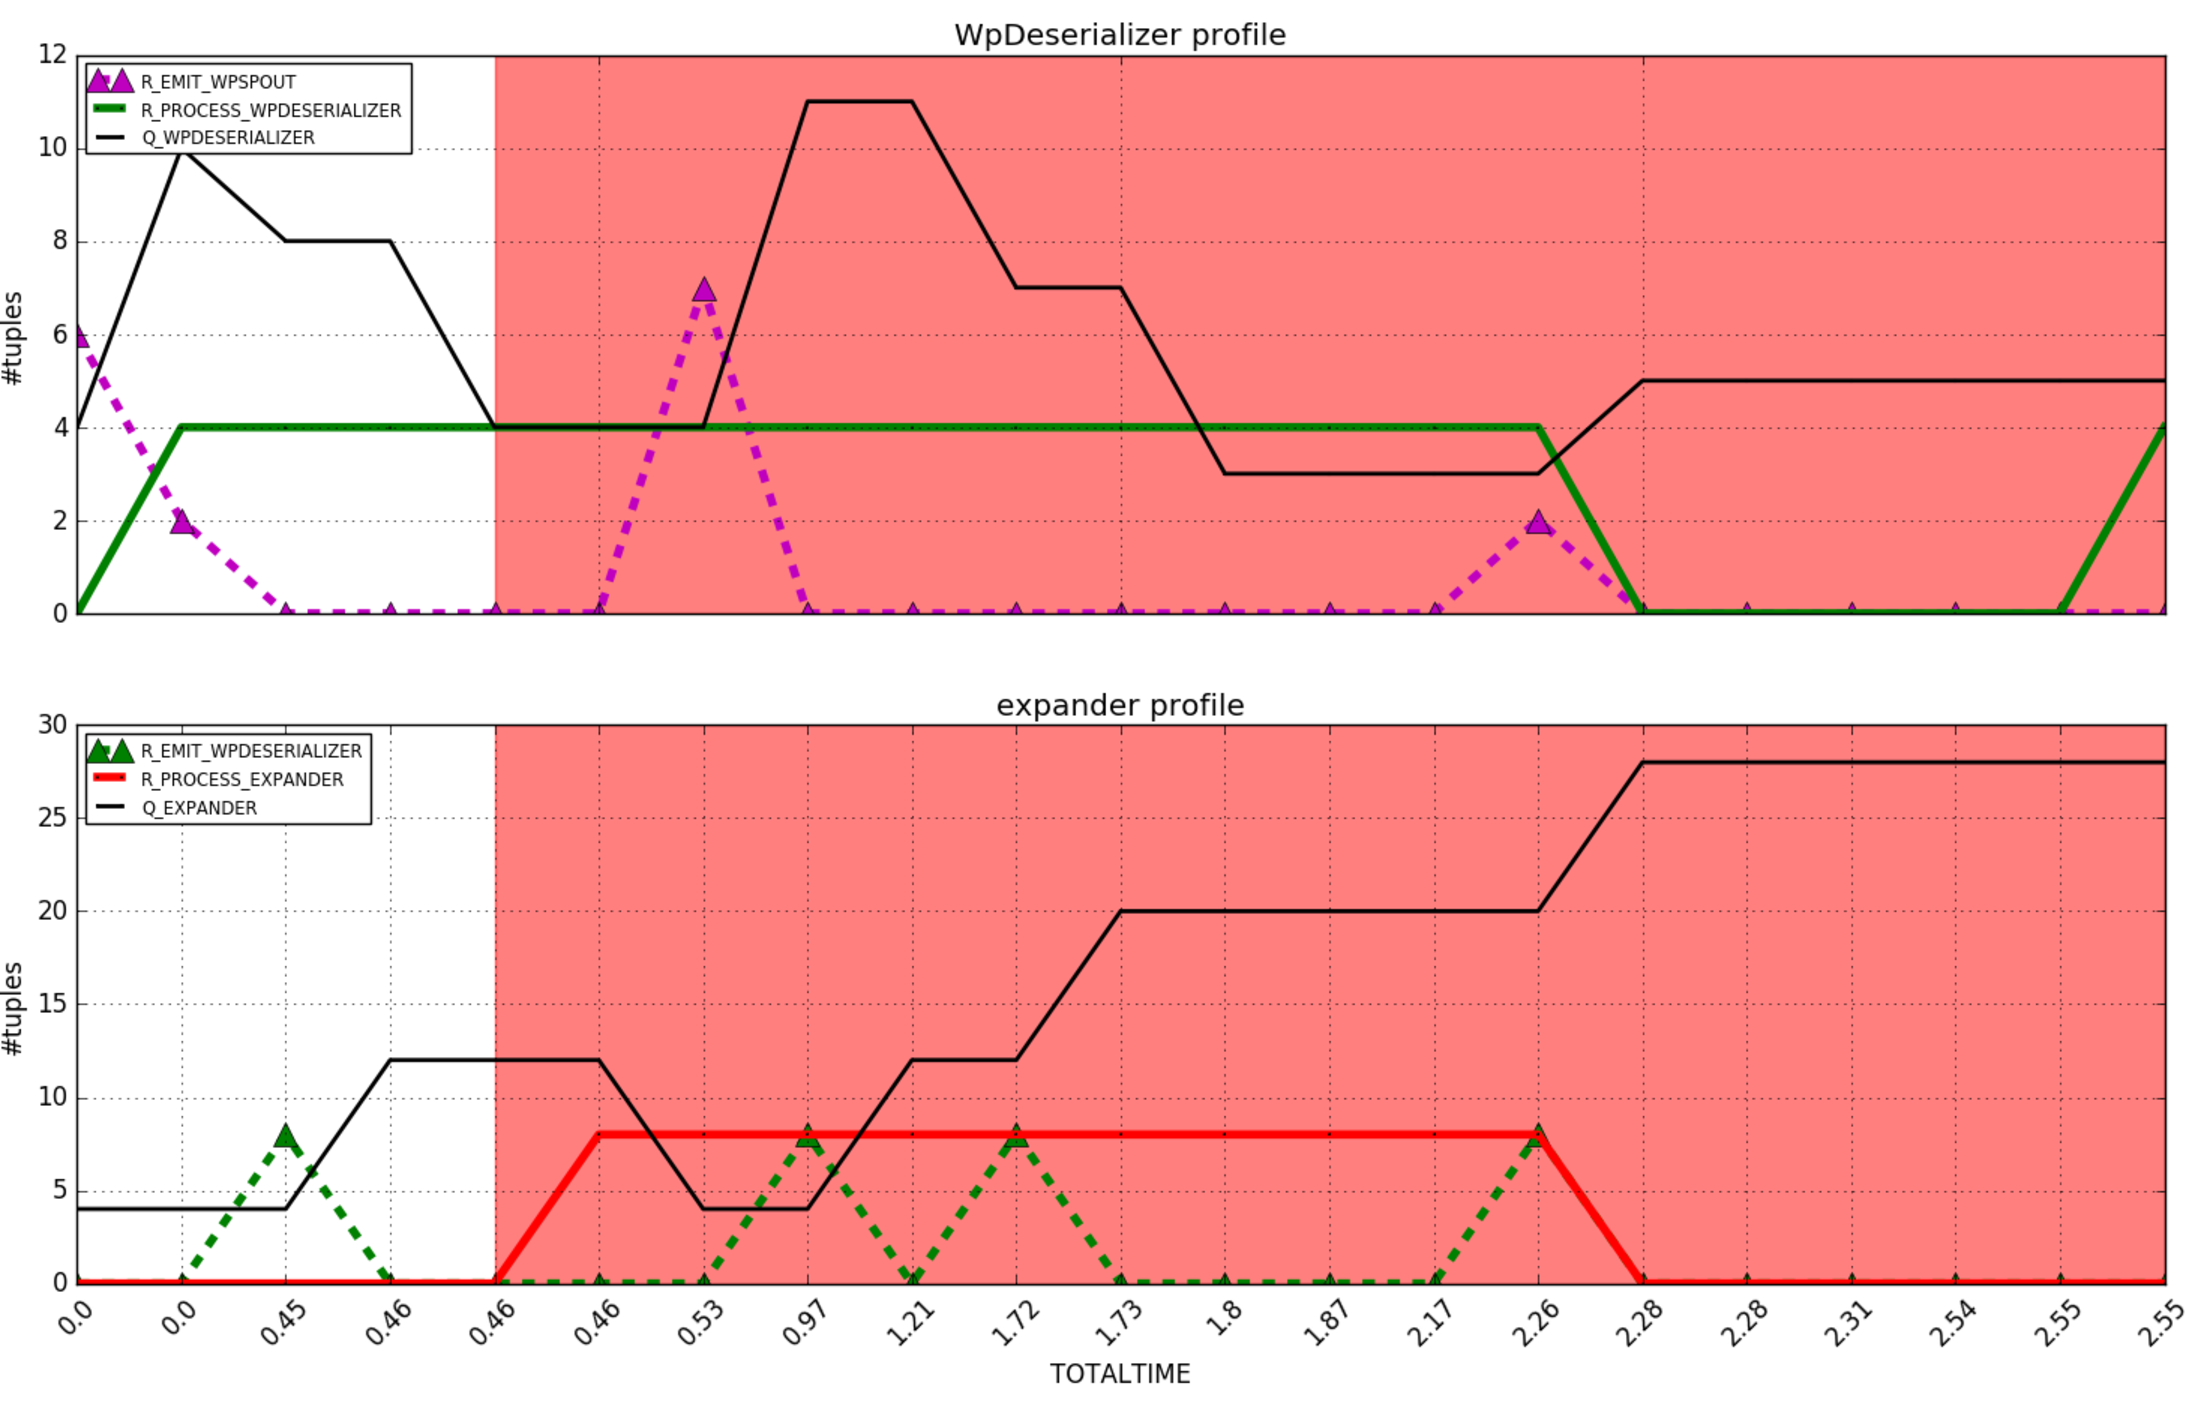
\includegraphics[width=1\linewidth]{images/verif-trace-color}
\caption{OSTIA-based formal verification output trace showing the evolution of the two bolts over time. Queue trends are displayed as solid black line. Green and red solid line show the processing activity of the bolts, while the dashed lines illustrate the incoming tuples from the subscribed nodes (\texttt{emit} events).}
\label{verif-trace}
\end{figure}

